\documentclass[1p]{elsarticle_modified}
%\bibliographystyle{elsarticle-num}

%\usepackage[colorlinks]{hyperref}
%\usepackage{abbrmath_seonhwa} %\Abb, \Ascr, \Acal ,\Abf, \Afrak
\usepackage{amsfonts}
\usepackage{amssymb}
\usepackage{amsmath}
\usepackage{amsthm}
\usepackage{scalefnt}
\usepackage{amsbsy}
\usepackage{kotex}
\usepackage{caption}
\usepackage{subfig}
\usepackage{color}
\usepackage{graphicx}
\usepackage{xcolor} %% white, black, red, green, blue, cyan, magenta, yellow
\usepackage{float}
\usepackage{setspace}
\usepackage{hyperref}

\usepackage{tikz}
\usetikzlibrary{arrows}

\usepackage{multirow}
\usepackage{array} % fixed length table
\usepackage{hhline}

%%%%%%%%%%%%%%%%%%%%%
\makeatletter
\renewcommand*\env@matrix[1][\arraystretch]{%
	\edef\arraystretch{#1}%
	\hskip -\arraycolsep
	\let\@ifnextchar\new@ifnextchar
	\array{*\c@MaxMatrixCols c}}
\makeatother %https://tex.stackexchange.com/questions/14071/how-can-i-increase-the-line-spacing-in-a-matrix
%%%%%%%%%%%%%%%

\usepackage[normalem]{ulem}

\newcommand{\msout}[1]{\ifmmode\text{\sout{\ensuremath{#1}}}\else\sout{#1}\fi}
%SOURCE: \msout is \stkout macro in https://tex.stackexchange.com/questions/20609/strikeout-in-math-mode

\newcommand{\cancel}[1]{
	\ifmmode
	{\color{red}\msout{#1}}
	\else
	{\color{red}\sout{#1}}
	\fi
}

\newcommand{\add}[1]{
	{\color{blue}\uwave{#1}}
}

\newcommand{\replace}[2]{
	\ifmmode
	{\color{red}\msout{#1}}{\color{blue}\uwave{#2}}
	\else
	{\color{red}\sout{#1}}{\color{blue}\uwave{#2}}
	\fi
}

\newcommand{\Sol}{\mathcal{S}} %segment
\newcommand{\D}{D} %diagram
\newcommand{\A}{\mathcal{A}} %arc


%%%%%%%%%%%%%%%%%%%%%%%%%%%%%5 test

\def\sl{\operatorname{\textup{SL}}(2,\Cbb)}
\def\psl{\operatorname{\textup{PSL}}(2,\Cbb)}
\def\quan{\mkern 1mu \triangleright \mkern 1mu}

\theoremstyle{definition}
\newtheorem{thm}{Theorem}[section]
\newtheorem{prop}[thm]{Proposition}
\newtheorem{lem}[thm]{Lemma}
\newtheorem{ques}[thm]{Question}
\newtheorem{cor}[thm]{Corollary}
\newtheorem{defn}[thm]{Definition}
\newtheorem{exam}[thm]{Example}
\newtheorem{rmk}[thm]{Remark}
\newtheorem{alg}[thm]{Algorithm}

\newcommand{\I}{\sqrt{-1}}
\begin{document}

%\begin{frontmatter}
%
%\title{Boundary parabolic representations of knots up to 8 crossings}
%
%%% Group authors per affiliation:
%\author{Yunhi Cho} 
%\address{Department of Mathematics, University of Seoul, Seoul, Korea}
%\ead{yhcho@uos.ac.kr}
%
%
%\author{Seonhwa Kim} %\fnref{s_kim}}
%\address{Center for Geometry and Physics, Institute for Basic Science, Pohang, 37673, Korea}
%\ead{ryeona17@ibs.re.kr}
%
%\author{Hyuk Kim}
%\address{Department of Mathematical Sciences, Seoul National University, Seoul 08826, Korea}
%\ead{hyukkim@snu.ac.kr}
%
%\author{Seokbeom Yoon}
%\address{Department of Mathematical Sciences, Seoul National University, Seoul, 08826,  Korea}
%\ead{sbyoon15@snu.ac.kr}
%
%\begin{abstract}
%We find all boundary parabolic representation of knots up to 8 crossings.
%
%\end{abstract}
%\begin{keyword}
%    \MSC[2010] 57M25 
%\end{keyword}
%
%\end{frontmatter}

%\linenumbers
%\tableofcontents
%
\newcommand\colored[1]{\textcolor{white}{\rule[-0.35ex]{0.8em}{1.4ex}}\kern-0.8em\color{red} #1}%
%\newcommand\colored[1]{\textcolor{white}{ #1}\kern-2.17ex	\textcolor{white}{ #1}\kern-1.81ex	\textcolor{white}{ #1}\kern-2.15ex\color{red}#1	}

{\Large $\underline{12n_{0341}~(K12n_{0341})}$}

\setlength{\tabcolsep}{10pt}
\renewcommand{\arraystretch}{1.6}
\vspace{1cm}\begin{tabular}{m{100pt}>{\centering\arraybackslash}m{274pt}}
\multirow{5}{120pt}{
	\centering
	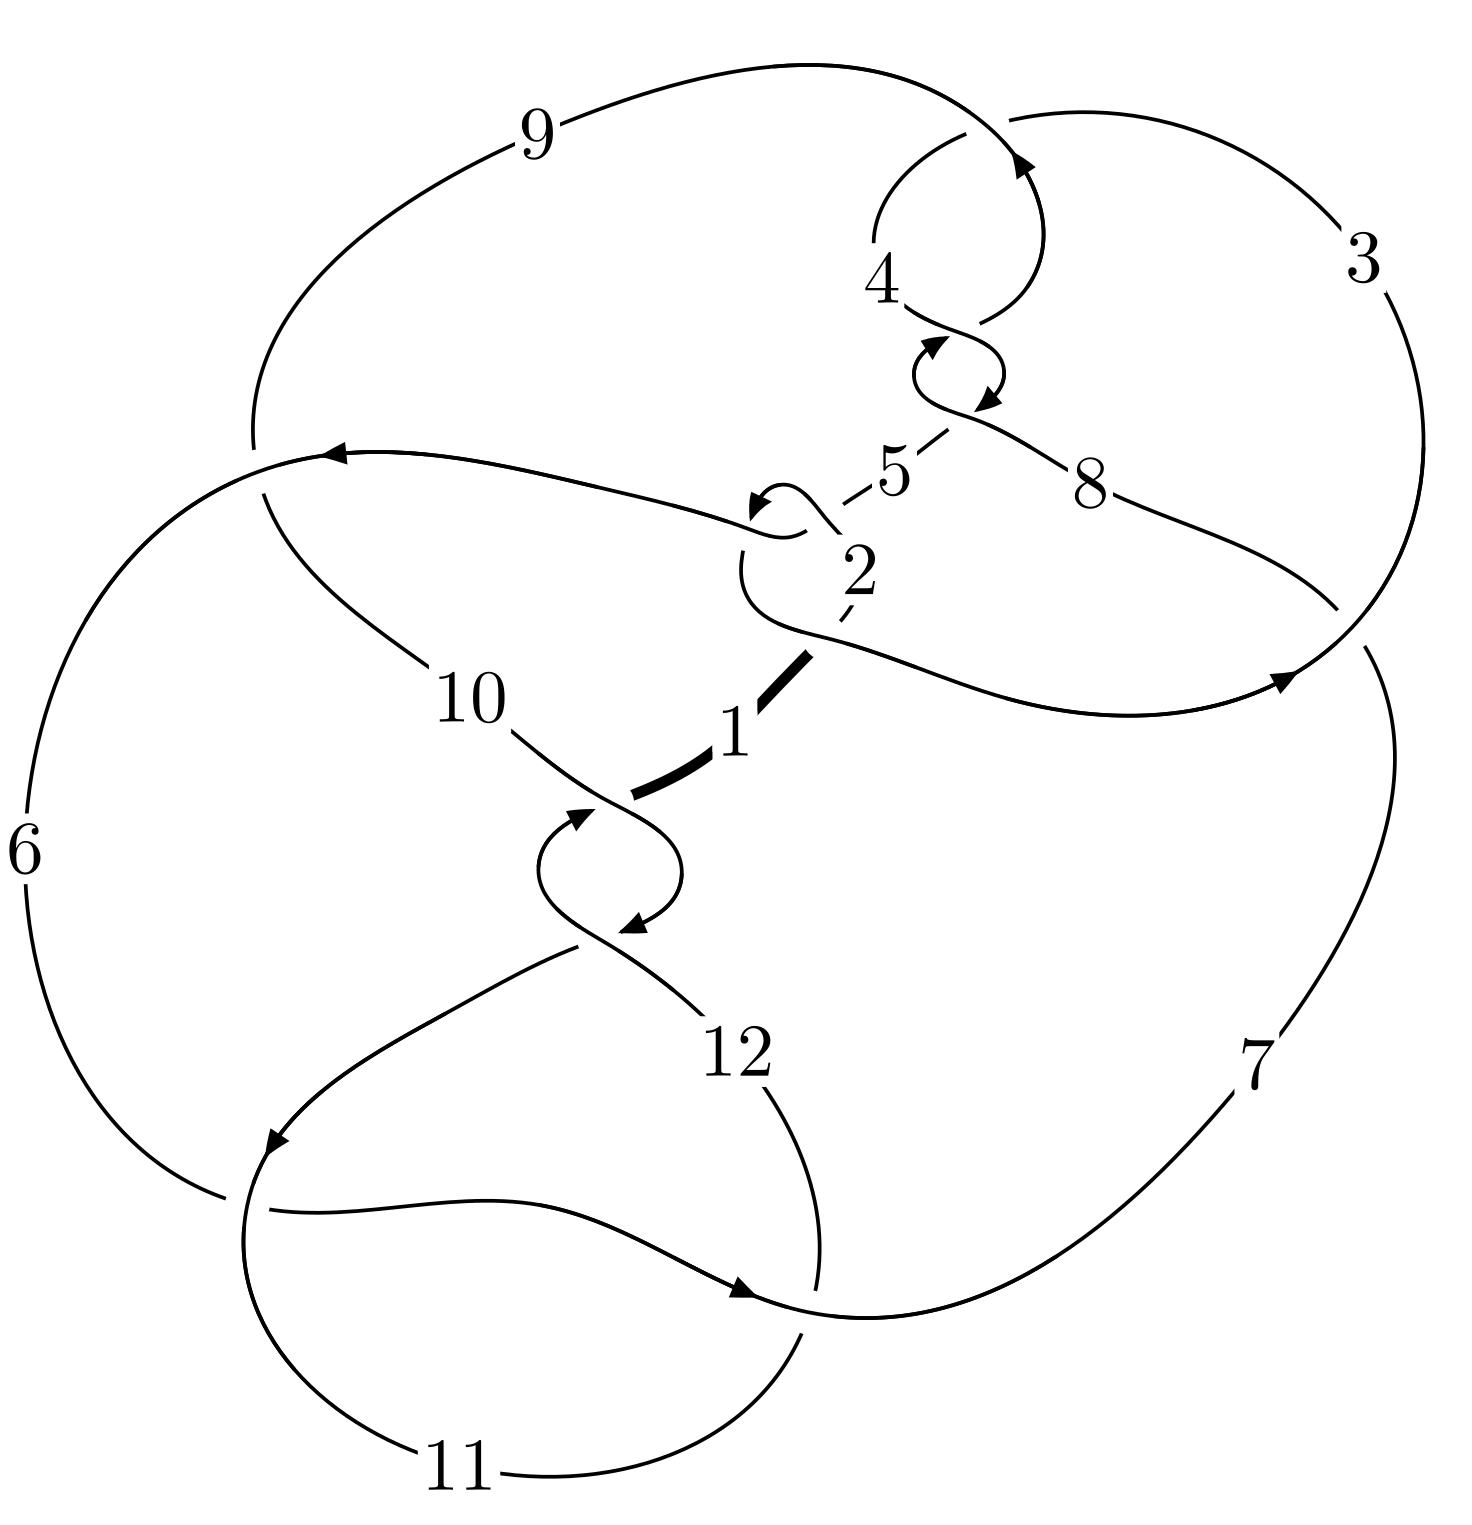
\includegraphics[width=112pt]{../../../GIT/diagram.site/Diagrams/png/2430_12n_0341.png}\\
\ \ \ A knot diagram\footnotemark}&
\allowdisplaybreaks
\textbf{Linearized knot diagam} \\
\cline{2-2}
 &
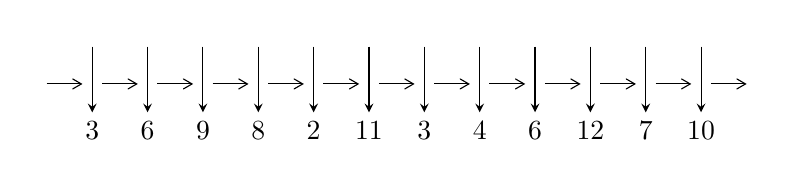
\begin{tikzpicture}[x=20pt, y=17pt]
	% nodes
	\node (C0) at (0, 0) {};
	\node (C1) at (1, 0) {};
	\node (C1U) at (1, +1) {};
	\node (C1D) at (1, -1) {3};

	\node (C2) at (2, 0) {};
	\node (C2U) at (2, +1) {};
	\node (C2D) at (2, -1) {6};

	\node (C3) at (3, 0) {};
	\node (C3U) at (3, +1) {};
	\node (C3D) at (3, -1) {9};

	\node (C4) at (4, 0) {};
	\node (C4U) at (4, +1) {};
	\node (C4D) at (4, -1) {8};

	\node (C5) at (5, 0) {};
	\node (C5U) at (5, +1) {};
	\node (C5D) at (5, -1) {2};

	\node (C6) at (6, 0) {};
	\node (C6U) at (6, +1) {};
	\node (C6D) at (6, -1) {11};

	\node (C7) at (7, 0) {};
	\node (C7U) at (7, +1) {};
	\node (C7D) at (7, -1) {3};

	\node (C8) at (8, 0) {};
	\node (C8U) at (8, +1) {};
	\node (C8D) at (8, -1) {4};

	\node (C9) at (9, 0) {};
	\node (C9U) at (9, +1) {};
	\node (C9D) at (9, -1) {6};

	\node (C10) at (10, 0) {};
	\node (C10U) at (10, +1) {};
	\node (C10D) at (10, -1) {12};

	\node (C11) at (11, 0) {};
	\node (C11U) at (11, +1) {};
	\node (C11D) at (11, -1) {7};

	\node (C12) at (12, 0) {};
	\node (C12U) at (12, +1) {};
	\node (C12D) at (12, -1) {10};
	\node (C13) at (13, 0) {};

	% arrows
	\draw[->,>={angle 60}]
	(C0) edge (C1) (C1) edge (C2) (C2) edge (C3) (C3) edge (C4) (C4) edge (C5) (C5) edge (C6) (C6) edge (C7) (C7) edge (C8) (C8) edge (C9) (C9) edge (C10) (C10) edge (C11) (C11) edge (C12) (C12) edge (C13) ;	\draw[->,>=stealth]
	(C1U) edge (C1D) (C2U) edge (C2D) (C3U) edge (C3D) (C4U) edge (C4D) (C5U) edge (C5D) (C6U) edge (C6D) (C7U) edge (C7D) (C8U) edge (C8D) (C9U) edge (C9D) (C10U) edge (C10D) (C11U) edge (C11D) (C12U) edge (C12D) ;
	\end{tikzpicture} \\
\hhline{~~} \\& 
\textbf{Solving Sequence} \\ \cline{2-2} 
 &
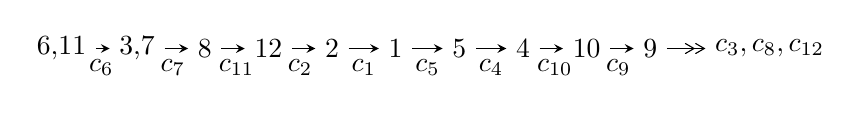
\begin{tikzpicture}[x=23pt, y=7pt]
	% node
	\node (A0) at (-1/8, 0) {6,11};
	\node (A1) at (17/16, 0) {3,7};
	\node (A2) at (17/8, 0) {8};
	\node (A3) at (25/8, 0) {12};
	\node (A4) at (33/8, 0) {2};
	\node (A5) at (41/8, 0) {1};
	\node (A6) at (49/8, 0) {5};
	\node (A7) at (57/8, 0) {4};
	\node (A8) at (65/8, 0) {10};
	\node (A9) at (73/8, 0) {9};
	\node (C1) at (1/2, -1) {$c_{6}$};
	\node (C2) at (13/8, -1) {$c_{7}$};
	\node (C3) at (21/8, -1) {$c_{11}$};
	\node (C4) at (29/8, -1) {$c_{2}$};
	\node (C5) at (37/8, -1) {$c_{1}$};
	\node (C6) at (45/8, -1) {$c_{5}$};
	\node (C7) at (53/8, -1) {$c_{4}$};
	\node (C8) at (61/8, -1) {$c_{10}$};
	\node (C9) at (69/8, -1) {$c_{9}$};
	\node (A10) at (11, 0) {$c_{3},c_{8},c_{12}$};

	% edge
	\draw[->,>=stealth]	
	(A0) edge (A1) (A1) edge (A2) (A2) edge (A3) (A3) edge (A4) (A4) edge (A5) (A5) edge (A6) (A6) edge (A7) (A7) edge (A8) (A8) edge (A9) ;
	\draw[->>,>={angle 60}]	
	(A9) edge (A10);
\end{tikzpicture} \\ 

\end{tabular} \\

\footnotetext{
The image of knot diagram is generated by the software ``\textbf{Draw programme}" developed by Andrew Bartholomew(\url{http://www.layer8.co.uk/maths/draw/index.htm\#Running-draw}), where we modified some parts for our purpose(\url{https://github.com/CATsTAILs/LinksPainter}).
}\phantom \\ \newline 
\centering \textbf{Ideals for irreducible components\footnotemark of $X_{\text{par}}$} 
 
\begin{align*}
I^u_{1}&=\langle 
7214350820 u^{41}+14261840536 u^{40}+\cdots+24614921861 b+13897246666,\\
\phantom{I^u_{1}}&\phantom{= \langle  }-286630329392 u^{41}+403439047669 u^{40}+\cdots+147689531166 a-913761324969,\\
\phantom{I^u_{1}}&\phantom{= \langle  }u^{42}-2 u^{41}+\cdots+3 u-3\rangle \\
I^u_{2}&=\langle 
b-1,\;a^2+2 a u+3 u^2-2 a-6 u+3,\;u^3- u^2+1\rangle \\
I^u_{3}&=\langle 
b+1,\;a+u+1,\;u^3+u^2-1\rangle \\
\\
\end{align*}
\raggedright * 3 irreducible components of $\dim_{\mathbb{C}}=0$, with total 51 representations.\\
\footnotetext{All coefficients of polynomials are rational numbers. But the coefficients are sometimes approximated in decimal forms when there is not enough margin.}
\newpage
\renewcommand{\arraystretch}{1}
\centering \section*{I. $I^u_{1}= \langle 7.21\times10^{9} u^{41}+1.43\times10^{10} u^{40}+\cdots+2.46\times10^{10} b+1.39\times10^{10},\;-2.87\times10^{11} u^{41}+4.03\times10^{11} u^{40}+\cdots+1.48\times10^{11} a-9.14\times10^{11},\;u^{42}-2 u^{41}+\cdots+3 u-3 \rangle$}
\flushleft \textbf{(i) Arc colorings}\\
\begin{tabular}{m{7pt} m{180pt} m{7pt} m{180pt} }
\flushright $a_{6}=$&$\begin{pmatrix}1\\0\end{pmatrix}$ \\
\flushright $a_{11}=$&$\begin{pmatrix}0\\u\end{pmatrix}$ \\
\flushright $a_{3}=$&$\begin{pmatrix}1.94076 u^{41}-2.73167 u^{40}+\cdots-1.14974 u+6.18704\\-0.293089 u^{41}-0.579398 u^{40}+\cdots+3.28574 u-0.564586\end{pmatrix}$ \\
\flushright $a_{7}=$&$\begin{pmatrix}1\\u^2\end{pmatrix}$ \\
\flushright $a_{8}=$&$\begin{pmatrix}-1.42423 u^{41}+1.18705 u^{40}+\cdots+4.86301 u+0.704689\\-1.16806 u^{41}+1.78911 u^{40}+\cdots-1.38926 u-3.49408\end{pmatrix}$ \\
\flushright $a_{12}=$&$\begin{pmatrix}- u\\- u^3+u\end{pmatrix}$ \\
\flushright $a_{2}=$&$\begin{pmatrix}1.64767 u^{41}-3.31107 u^{40}+\cdots+2.13601 u+5.62246\\-0.293089 u^{41}-0.579398 u^{40}+\cdots+3.28574 u-0.564586\end{pmatrix}$ \\
\flushright $a_{1}=$&$\begin{pmatrix}- u^5- u\\- u^7+u^5-2 u^3+u\end{pmatrix}$ \\
\flushright $a_{5}=$&$\begin{pmatrix}-1.90746 u^{41}+4.07002 u^{40}+\cdots-4.13107 u-3.28175\\0.164081 u^{41}+0.812895 u^{40}+\cdots-2.16751 u+0.836225\end{pmatrix}$ \\
\flushright $a_{4}=$&$\begin{pmatrix}1.43869 u^{41}-0.929160 u^{40}+\cdots-3.24612 u+9.35450\\-0.222585 u^{41}+0.354594 u^{40}+\cdots+1.79645 u+0.987097\end{pmatrix}$ \\
\flushright $a_{10}=$&$\begin{pmatrix}u^3\\u^5- u^3+u\end{pmatrix}$ \\
\flushright $a_{9}=$&$\begin{pmatrix}u^5+u\\u^5- u^3+u\end{pmatrix}$\\&\end{tabular}
\flushleft \textbf{(ii) Obstruction class $= -1$}\\~\\
\flushleft \textbf{(iii) Cusp Shapes $= -\frac{47220782375}{24614921861} u^{41}-\frac{499793100}{24614921861} u^{40}+\cdots+\frac{450722117512}{24614921861} u-\frac{698025687495}{24614921861}$}\\~\\
\newpage\renewcommand{\arraystretch}{1}
\flushleft \textbf{(iv) u-Polynomials at the component}\newline \\
\begin{tabular}{m{50pt}|m{274pt}}
Crossings & \hspace{64pt}u-Polynomials at each crossing \\
\hline $$\begin{aligned}c_{1}\end{aligned}$$&$\begin{aligned}
&u^{42}+50 u^{41}+\cdots-190 u+1
\end{aligned}$\\
\hline $$\begin{aligned}c_{2},c_{5}\end{aligned}$$&$\begin{aligned}
&u^{42}+4 u^{41}+\cdots+12 u-1
\end{aligned}$\\
\hline $$\begin{aligned}c_{3},c_{4},c_{8}\end{aligned}$$&$\begin{aligned}
&u^{42}+u^{41}+\cdots+16 u+8
\end{aligned}$\\
\hline $$\begin{aligned}c_{6},c_{11}\end{aligned}$$&$\begin{aligned}
&u^{42}-2 u^{41}+\cdots+3 u-3
\end{aligned}$\\
\hline $$\begin{aligned}c_{7}\end{aligned}$$&$\begin{aligned}
&u^{42}- u^{41}+\cdots+64 u+8
\end{aligned}$\\
\hline $$\begin{aligned}c_{9}\end{aligned}$$&$\begin{aligned}
&u^{42}+2 u^{41}+\cdots+15 u-3
\end{aligned}$\\
\hline $$\begin{aligned}c_{10},c_{12}\end{aligned}$$&$\begin{aligned}
&u^{42}+16 u^{41}+\cdots+147 u+9
\end{aligned}$\\
\hline
\end{tabular}\\~\\
\newpage\renewcommand{\arraystretch}{1}
\flushleft \textbf{(v) Riley Polynomials at the component}\newline \\
\begin{tabular}{m{50pt}|m{274pt}}
Crossings & \hspace{64pt}Riley Polynomials at each crossing \\
\hline $$\begin{aligned}c_{1}\end{aligned}$$&$\begin{aligned}
&y^{42}-106 y^{41}+\cdots+9510 y+1
\end{aligned}$\\
\hline $$\begin{aligned}c_{2},c_{5}\end{aligned}$$&$\begin{aligned}
&y^{42}-50 y^{41}+\cdots+190 y+1
\end{aligned}$\\
\hline $$\begin{aligned}c_{3},c_{4},c_{8}\end{aligned}$$&$\begin{aligned}
&y^{42}+35 y^{41}+\cdots+128 y+64
\end{aligned}$\\
\hline $$\begin{aligned}c_{6},c_{11}\end{aligned}$$&$\begin{aligned}
&y^{42}-16 y^{41}+\cdots-147 y+9
\end{aligned}$\\
\hline $$\begin{aligned}c_{7}\end{aligned}$$&$\begin{aligned}
&y^{42}-49 y^{41}+\cdots+1536 y+64
\end{aligned}$\\
\hline $$\begin{aligned}c_{9}\end{aligned}$$&$\begin{aligned}
&y^{42}-48 y^{41}+\cdots-3 y+9
\end{aligned}$\\
\hline $$\begin{aligned}c_{10},c_{12}\end{aligned}$$&$\begin{aligned}
&y^{42}+24 y^{41}+\cdots-2367 y+81
\end{aligned}$\\
\hline
\end{tabular}\\~\\
\newpage\flushleft \textbf{(vi) Complex Volumes and Cusp Shapes}
$$\begin{array}{c|c|c}  
\text{Solutions to }I^u_{1}& \I (\text{vol} + \sqrt{-1}CS) & \text{Cusp shape}\\
 \hline 
\begin{aligned}
u &= -0.493349 + 0.873287 I \\
a &= \phantom{-}0.358491 - 0.000809 I \\
b &= \phantom{-}1.62688 + 0.12135 I\end{aligned}
 & -7.72387 - 2.08243 I & -13.63208 + 0.61844 I \\ \hline\begin{aligned}
u &= -0.493349 - 0.873287 I \\
a &= \phantom{-}0.358491 + 0.000809 I \\
b &= \phantom{-}1.62688 - 0.12135 I\end{aligned}
 & -7.72387 + 2.08243 I & -13.63208 - 0.61844 I \\ \hline\begin{aligned}
u &= -0.857671 + 0.547734 I \\
a &= \phantom{-}2.39738 + 0.56265 I \\
b &= \phantom{-}1.297890 + 0.093808 I\end{aligned}
 & \phantom{-}3.74220 + 2.19658 I & -11.88073 - 3.02970 I \\ \hline\begin{aligned}
u &= -0.857671 - 0.547734 I \\
a &= \phantom{-}2.39738 - 0.56265 I \\
b &= \phantom{-}1.297890 - 0.093808 I\end{aligned}
 & \phantom{-}3.74220 - 2.19658 I & -11.88073 + 3.02970 I \\ \hline\begin{aligned}
u &= -1.042580 + 0.004634 I \\
a &= \phantom{-}1.183060 + 0.451877 I \\
b &= \phantom{-}0.711272 + 0.677400 I\end{aligned}
 & -1.44341 - 2.30270 I & -14.7058 + 3.7232 I \\ \hline\begin{aligned}
u &= -1.042580 - 0.004634 I \\
a &= \phantom{-}1.183060 - 0.451877 I \\
b &= \phantom{-}0.711272 - 0.677400 I\end{aligned}
 & -1.44341 + 2.30270 I & -14.7058 - 3.7232 I \\ \hline\begin{aligned}
u &= \phantom{-}0.586636 + 0.736989 I \\
a &= -0.267637 + 0.708323 I \\
b &= \phantom{-}0.487231 - 0.786141 I\end{aligned}
 & \phantom{-}3.87323 + 3.15388 I & -7.00575 - 3.01303 I \\ \hline\begin{aligned}
u &= \phantom{-}0.586636 - 0.736989 I \\
a &= -0.267637 - 0.708323 I \\
b &= \phantom{-}0.487231 + 0.786141 I\end{aligned}
 & \phantom{-}3.87323 - 3.15388 I & -7.00575 + 3.01303 I \\ \hline\begin{aligned}
u &= \phantom{-}0.587628 + 0.887835 I \\
a &= -0.300671 - 0.305913 I \\
b &= -1.57989 + 0.27896 I\end{aligned}
 & -3.00105 + 7.12424 I & -10.18276 - 2.97506 I \\ \hline\begin{aligned}
u &= \phantom{-}0.587628 - 0.887835 I \\
a &= -0.300671 + 0.305913 I \\
b &= -1.57989 - 0.27896 I\end{aligned}
 & -3.00105 - 7.12424 I & -10.18276 + 2.97506 I\\
 \hline 
 \end{array}$$\newpage$$\begin{array}{c|c|c}  
\text{Solutions to }I^u_{1}& \I (\text{vol} + \sqrt{-1}CS) & \text{Cusp shape}\\
 \hline 
\begin{aligned}
u &= \phantom{-}0.893636 + 0.236079 I \\
a &= -1.66259 + 0.50310 I \\
b &= -1.141660 + 0.275387 I\end{aligned}
 & -3.22132 - 0.72709 I & -17.2502 + 5.7568 I \\ \hline\begin{aligned}
u &= \phantom{-}0.893636 - 0.236079 I \\
a &= -1.66259 - 0.50310 I \\
b &= -1.141660 - 0.275387 I\end{aligned}
 & -3.22132 + 0.72709 I & -17.2502 - 5.7568 I \\ \hline\begin{aligned}
u &= \phantom{-}0.364728 + 0.832070 I \\
a &= -0.385710 + 0.359680 I \\
b &= -1.59824 - 0.07981 I\end{aligned}
 & -4.34661 - 3.12224 I & -10.84272 + 2.92675 I \\ \hline\begin{aligned}
u &= \phantom{-}0.364728 - 0.832070 I \\
a &= -0.385710 - 0.359680 I \\
b &= -1.59824 + 0.07981 I\end{aligned}
 & -4.34661 + 3.12224 I & -10.84272 - 2.92675 I \\ \hline\begin{aligned}
u &= \phantom{-}0.878925 + 0.694557 I \\
a &= \phantom{-}0.310415 - 0.409583 I \\
b &= \phantom{-}0.590948 - 0.108791 I\end{aligned}
 & \phantom{-}2.08568 - 2.67535 I & -4.92251 + 2.20937 I \\ \hline\begin{aligned}
u &= \phantom{-}0.878925 - 0.694557 I \\
a &= \phantom{-}0.310415 + 0.409583 I \\
b &= \phantom{-}0.590948 + 0.108791 I\end{aligned}
 & \phantom{-}2.08568 + 2.67535 I & -4.92251 - 2.20937 I \\ \hline\begin{aligned}
u &= \phantom{-}0.949655 + 0.594867 I \\
a &= -0.255068 - 0.352987 I \\
b &= \phantom{-}0.662783 - 0.635045 I\end{aligned}
 & \phantom{-}2.08502 - 3.11024 I & -10.10897 + 3.32337 I \\ \hline\begin{aligned}
u &= \phantom{-}0.949655 - 0.594867 I \\
a &= -0.255068 + 0.352987 I \\
b &= \phantom{-}0.662783 + 0.635045 I\end{aligned}
 & \phantom{-}2.08502 + 3.11024 I & -10.10897 - 3.32337 I \\ \hline\begin{aligned}
u &= -0.967079 + 0.570637 I \\
a &= -1.10245 - 1.08422 I \\
b &= -0.758887 + 0.665919 I\end{aligned}
 & -1.15338 + 4.42053 I & -14.9758 - 5.6521 I \\ \hline\begin{aligned}
u &= -0.967079 - 0.570637 I \\
a &= -1.10245 + 1.08422 I \\
b &= -0.758887 - 0.665919 I\end{aligned}
 & -1.15338 - 4.42053 I & -14.9758 + 5.6521 I\\
 \hline 
 \end{array}$$\newpage$$\begin{array}{c|c|c}  
\text{Solutions to }I^u_{1}& \I (\text{vol} + \sqrt{-1}CS) & \text{Cusp shape}\\
 \hline 
\begin{aligned}
u &= \phantom{-}0.739578 + 0.450680 I \\
a &= \phantom{-}0.34684 - 1.84376 I \\
b &= \phantom{-}0.854538 + 0.412162 I\end{aligned}
 & \phantom{-}2.96029 - 1.36479 I & -9.90879 + 4.47886 I \\ \hline\begin{aligned}
u &= \phantom{-}0.739578 - 0.450680 I \\
a &= \phantom{-}0.34684 + 1.84376 I \\
b &= \phantom{-}0.854538 - 0.412162 I\end{aligned}
 & \phantom{-}2.96029 + 1.36479 I & -9.90879 - 4.47886 I \\ \hline\begin{aligned}
u &= -0.870477 + 0.749362 I \\
a &= -0.989419 + 0.125741 I \\
b &= \phantom{-}0.0326402 - 0.0700810 I\end{aligned}
 & \phantom{-}7.96823 + 2.83809 I & -2.44683 - 2.99950 I \\ \hline\begin{aligned}
u &= -0.870477 - 0.749362 I \\
a &= -0.989419 - 0.125741 I \\
b &= \phantom{-}0.0326402 + 0.0700810 I\end{aligned}
 & \phantom{-}7.96823 - 2.83809 I & -2.44683 + 2.99950 I \\ \hline\begin{aligned}
u &= -0.667718 + 0.509431 I \\
a &= \phantom{-}0.526984 + 0.298925 I \\
b &= -0.455324 - 0.527591 I\end{aligned}
 & -0.215927 + 0.057739 I & -12.86905 + 0.99724 I \\ \hline\begin{aligned}
u &= -0.667718 - 0.509431 I \\
a &= \phantom{-}0.526984 - 0.298925 I \\
b &= -0.455324 + 0.527591 I\end{aligned}
 & -0.215927 - 0.057739 I & -12.86905 - 0.99724 I \\ \hline\begin{aligned}
u &= -1.192640 + 0.084412 I \\
a &= -2.72686 - 0.35998 I \\
b &= -1.68766 + 0.19280 I\end{aligned}
 & -9.82219 + 5.69889 I & -16.0238 - 3.4541 I \\ \hline\begin{aligned}
u &= -1.192640 - 0.084412 I \\
a &= -2.72686 + 0.35998 I \\
b &= -1.68766 - 0.19280 I\end{aligned}
 & -9.82219 - 5.69889 I & -16.0238 + 3.4541 I \\ \hline\begin{aligned}
u &= \phantom{-}1.20918\phantom{ +0.000000I} \\
a &= \phantom{-}2.73290\phantom{ +0.000000I} \\
b &= \phantom{-}1.73917\phantom{ +0.000000I}\end{aligned}
 & -13.9658\phantom{ +0.000000I} & -18.7010\phantom{ +0.000000I} \\ \hline\begin{aligned}
u &= -0.893982 + 0.823604 I \\
a &= \phantom{-}0.017481 - 0.836922 I \\
b &= -1.322530 + 0.004918 I\end{aligned}
 & \phantom{-}3.39487 + 3.06804 I & -10.44365 - 2.87354 I\\
 \hline 
 \end{array}$$\newpage$$\begin{array}{c|c|c}  
\text{Solutions to }I^u_{1}& \I (\text{vol} + \sqrt{-1}CS) & \text{Cusp shape}\\
 \hline 
\begin{aligned}
u &= -0.893982 - 0.823604 I \\
a &= \phantom{-}0.017481 + 0.836922 I \\
b &= -1.322530 - 0.004918 I\end{aligned}
 & \phantom{-}3.39487 - 3.06804 I & -10.44365 + 2.87354 I \\ \hline\begin{aligned}
u &= \phantom{-}1.029980 + 0.651441 I \\
a &= \phantom{-}1.19267 - 0.82522 I \\
b &= \phantom{-}0.548001 + 0.888471 I\end{aligned}
 & \phantom{-}2.56002 - 8.46686 I & -9.68679 + 7.74880 I \\ \hline\begin{aligned}
u &= \phantom{-}1.029980 - 0.651441 I \\
a &= \phantom{-}1.19267 + 0.82522 I \\
b &= \phantom{-}0.548001 - 0.888471 I\end{aligned}
 & \phantom{-}2.56002 + 8.46686 I & -9.68679 - 7.74880 I \\ \hline\begin{aligned}
u &= \phantom{-}1.106730 + 0.589792 I \\
a &= -1.63532 + 1.44131 I \\
b &= -1.67176 - 0.00321 I\end{aligned}
 & -6.57334 - 2.08658 I & -13.90990 + 1.57056 I \\ \hline\begin{aligned}
u &= \phantom{-}1.106730 - 0.589792 I \\
a &= -1.63532 - 1.44131 I \\
b &= -1.67176 + 0.00321 I\end{aligned}
 & -6.57334 + 2.08658 I & -13.90990 - 1.57056 I \\ \hline\begin{aligned}
u &= -1.107090 + 0.662634 I \\
a &= \phantom{-}1.51861 + 1.67496 I \\
b &= \phantom{-}1.68068 - 0.19305 I\end{aligned}
 & -9.58882 + 7.76603 I & -15.5418 - 5.0561 I \\ \hline\begin{aligned}
u &= -1.107090 - 0.662634 I \\
a &= \phantom{-}1.51861 - 1.67496 I \\
b &= \phantom{-}1.68068 + 0.19305 I\end{aligned}
 & -9.58882 - 7.76603 I & -15.5418 + 5.0561 I \\ \hline\begin{aligned}
u &= \phantom{-}1.084910 + 0.710010 I \\
a &= -1.42076 + 1.88196 I \\
b &= -1.60580 - 0.32883 I\end{aligned}
 & -4.52539 - 13.04420 I & -12.00000 + 7.21592 I \\ \hline\begin{aligned}
u &= \phantom{-}1.084910 - 0.710010 I \\
a &= -1.42076 - 1.88196 I \\
b &= -1.60580 + 0.32883 I\end{aligned}
 & -4.52539 + 13.04420 I & -12.00000 - 7.21592 I \\ \hline\begin{aligned}
u &= \phantom{-}0.451064 + 0.481038 I \\
a &= -0.346528 - 1.234360 I \\
b &= \phantom{-}0.610635 + 0.462564 I\end{aligned}
 & \phantom{-}3.08466 - 1.37137 I & -7.10497 + 4.42267 I\\
 \hline 
 \end{array}$$\newpage$$\begin{array}{c|c|c}  
\text{Solutions to }I^u_{1}& \I (\text{vol} + \sqrt{-1}CS) & \text{Cusp shape}\\
 \hline 
\begin{aligned}
u &= \phantom{-}0.451064 - 0.481038 I \\
a &= -0.346528 + 1.234360 I \\
b &= \phantom{-}0.610635 - 0.462564 I\end{aligned}
 & \phantom{-}3.08466 + 1.37137 I & -7.10497 - 4.42267 I \\ \hline\begin{aligned}
u &= -0.370951\phantom{ +0.000000I} \\
a &= \phantom{-}0.749235\phantom{ +0.000000I} \\
b &= -0.302638\phantom{ +0.000000I}\end{aligned}
 & -0.594790\phantom{ +0.000000I} & -16.5260\phantom{ +0.000000I}\\
 \hline 
 \end{array}$$\newpage\newpage\renewcommand{\arraystretch}{1}
\centering \section*{II. $I^u_{2}= \langle b-1,\;a^2+2 a u+3 u^2-2 a-6 u+3,\;u^3- u^2+1 \rangle$}
\flushleft \textbf{(i) Arc colorings}\\
\begin{tabular}{m{7pt} m{180pt} m{7pt} m{180pt} }
\flushright $a_{6}=$&$\begin{pmatrix}1\\0\end{pmatrix}$ \\
\flushright $a_{11}=$&$\begin{pmatrix}0\\u\end{pmatrix}$ \\
\flushright $a_{3}=$&$\begin{pmatrix}a\\1\end{pmatrix}$ \\
\flushright $a_{7}=$&$\begin{pmatrix}1\\u^2\end{pmatrix}$ \\
\flushright $a_{8}=$&$\begin{pmatrix}- a-3 u+4\\- u^2 a+u^2+1\end{pmatrix}$ \\
\flushright $a_{12}=$&$\begin{pmatrix}- u\\- u^2+u+1\end{pmatrix}$ \\
\flushright $a_{2}=$&$\begin{pmatrix}a+1\\1\end{pmatrix}$ \\
\flushright $a_{1}=$&$\begin{pmatrix}1\\0\end{pmatrix}$ \\
\flushright $a_{5}=$&$\begin{pmatrix}- a\\-1\end{pmatrix}$ \\
\flushright $a_{4}=$&$\begin{pmatrix}u^2 a+a-1\\u^2 a- a u- u^2- a+1\end{pmatrix}$ \\
\flushright $a_{10}=$&$\begin{pmatrix}u^2-1\\- u^2\end{pmatrix}$ \\
\flushright $a_{9}=$&$\begin{pmatrix}-1\\- u^2\end{pmatrix}$\\&\end{tabular}
\flushleft \textbf{(ii) Obstruction class $= 1$}\\~\\
\flushleft \textbf{(iii) Cusp Shapes $= 4 u-12$}\\~\\
\newpage\renewcommand{\arraystretch}{1}
\flushleft \textbf{(iv) u-Polynomials at the component}\newline \\
\begin{tabular}{m{50pt}|m{274pt}}
Crossings & \hspace{64pt}u-Polynomials at each crossing \\
\hline $$\begin{aligned}c_{1},c_{5}\end{aligned}$$&$\begin{aligned}
&(u-1)^6
\end{aligned}$\\
\hline $$\begin{aligned}c_{2}\end{aligned}$$&$\begin{aligned}
&(u+1)^6
\end{aligned}$\\
\hline $$\begin{aligned}c_{3},c_{4},c_{7}\\c_{8}\end{aligned}$$&$\begin{aligned}
&(u^2+2)^3
\end{aligned}$\\
\hline $$\begin{aligned}c_{6}\end{aligned}$$&$\begin{aligned}
&(u^3- u^2+1)^2
\end{aligned}$\\
\hline $$\begin{aligned}c_{9},c_{10}\end{aligned}$$&$\begin{aligned}
&(u^3- u^2+2 u-1)^2
\end{aligned}$\\
\hline $$\begin{aligned}c_{11}\end{aligned}$$&$\begin{aligned}
&(u^3+u^2-1)^2
\end{aligned}$\\
\hline $$\begin{aligned}c_{12}\end{aligned}$$&$\begin{aligned}
&(u^3+u^2+2 u+1)^2
\end{aligned}$\\
\hline
\end{tabular}\\~\\
\newpage\renewcommand{\arraystretch}{1}
\flushleft \textbf{(v) Riley Polynomials at the component}\newline \\
\begin{tabular}{m{50pt}|m{274pt}}
Crossings & \hspace{64pt}Riley Polynomials at each crossing \\
\hline $$\begin{aligned}c_{1},c_{2},c_{5}\end{aligned}$$&$\begin{aligned}
&(y-1)^6
\end{aligned}$\\
\hline $$\begin{aligned}c_{3},c_{4},c_{7}\\c_{8}\end{aligned}$$&$\begin{aligned}
&(y+2)^6
\end{aligned}$\\
\hline $$\begin{aligned}c_{6},c_{11}\end{aligned}$$&$\begin{aligned}
&(y^3- y^2+2 y-1)^2
\end{aligned}$\\
\hline $$\begin{aligned}c_{9},c_{10},c_{12}\end{aligned}$$&$\begin{aligned}
&(y^3+3 y^2+2 y-1)^2
\end{aligned}$\\
\hline
\end{tabular}\\~\\
\newpage\flushleft \textbf{(vi) Complex Volumes and Cusp Shapes}
$$\begin{array}{c|c|c}  
\text{Solutions to }I^u_{2}& \I (\text{vol} + \sqrt{-1}CS) & \text{Cusp shape}\\
 \hline 
\begin{aligned}
u &= \phantom{-}0.877439 + 0.744862 I \\
a &= \phantom{-}1.175960 - 0.571534 I \\
b &= \phantom{-}1.00000\phantom{ +0.000000I}\end{aligned}
 & \phantom{-}6.31400 - 2.82812 I & -8.49024 + 2.97945 I \\ \hline\begin{aligned}
u &= \phantom{-}0.877439 + 0.744862 I \\
a &= -0.930832 - 0.918189 I \\
b &= \phantom{-}1.00000\phantom{ +0.000000I}\end{aligned}
 & \phantom{-}6.31400 - 2.82812 I & -8.49024 + 2.97945 I \\ \hline\begin{aligned}
u &= \phantom{-}0.877439 - 0.744862 I \\
a &= \phantom{-}1.175960 + 0.571534 I \\
b &= \phantom{-}1.00000\phantom{ +0.000000I}\end{aligned}
 & \phantom{-}6.31400 + 2.82812 I & -8.49024 - 2.97945 I \\ \hline\begin{aligned}
u &= \phantom{-}0.877439 - 0.744862 I \\
a &= -0.930832 + 0.918189 I \\
b &= \phantom{-}1.00000\phantom{ +0.000000I}\end{aligned}
 & \phantom{-}6.31400 + 2.82812 I & -8.49024 - 2.97945 I \\ \hline\begin{aligned}
u &= -0.754878\phantom{ +0.000000I} \\
a &= \phantom{-}1.75488 + 2.48177 I \\
b &= \phantom{-}1.00000\phantom{ +0.000000I}\end{aligned}
 & \phantom{-}2.17641\phantom{ +0.000000I} & -15.0200\phantom{ +0.000000I} \\ \hline\begin{aligned}
u &= -0.754878\phantom{ +0.000000I} \\
a &= \phantom{-}1.75488 - 2.48177 I \\
b &= \phantom{-}1.00000\phantom{ +0.000000I}\end{aligned}
 & \phantom{-}2.17641\phantom{ +0.000000I} & -15.0200\phantom{ +0.000000I}\\
 \hline 
 \end{array}$$\newpage\newpage\renewcommand{\arraystretch}{1}
\centering \section*{III. $I^u_{3}= \langle b+1,\;a+u+1,\;u^3+u^2-1 \rangle$}
\flushleft \textbf{(i) Arc colorings}\\
\begin{tabular}{m{7pt} m{180pt} m{7pt} m{180pt} }
\flushright $a_{6}=$&$\begin{pmatrix}1\\0\end{pmatrix}$ \\
\flushright $a_{11}=$&$\begin{pmatrix}0\\u\end{pmatrix}$ \\
\flushright $a_{3}=$&$\begin{pmatrix}- u-1\\-1\end{pmatrix}$ \\
\flushright $a_{7}=$&$\begin{pmatrix}1\\u^2\end{pmatrix}$ \\
\flushright $a_{8}=$&$\begin{pmatrix}1\\u^2\end{pmatrix}$ \\
\flushright $a_{12}=$&$\begin{pmatrix}- u\\u^2+u-1\end{pmatrix}$ \\
\flushright $a_{2}=$&$\begin{pmatrix}- u-2\\-1\end{pmatrix}$ \\
\flushright $a_{1}=$&$\begin{pmatrix}-1\\0\end{pmatrix}$ \\
\flushright $a_{5}=$&$\begin{pmatrix}- u-1\\-1\end{pmatrix}$ \\
\flushright $a_{4}=$&$\begin{pmatrix}- u-1\\-1\end{pmatrix}$ \\
\flushright $a_{10}=$&$\begin{pmatrix}- u^2+1\\u^2\end{pmatrix}$ \\
\flushright $a_{9}=$&$\begin{pmatrix}1\\u^2\end{pmatrix}$\\&\end{tabular}
\flushleft \textbf{(ii) Obstruction class $= 1$}\\~\\
\flushleft \textbf{(iii) Cusp Shapes $= 4 u^2+2 u-16$}\\~\\
\newpage\renewcommand{\arraystretch}{1}
\flushleft \textbf{(iv) u-Polynomials at the component}\newline \\
\begin{tabular}{m{50pt}|m{274pt}}
Crossings & \hspace{64pt}u-Polynomials at each crossing \\
\hline $$\begin{aligned}c_{1},c_{2}\end{aligned}$$&$\begin{aligned}
&(u-1)^3
\end{aligned}$\\
\hline $$\begin{aligned}c_{3},c_{4},c_{7}\\c_{8}\end{aligned}$$&$\begin{aligned}
&u^3
\end{aligned}$\\
\hline $$\begin{aligned}c_{5}\end{aligned}$$&$\begin{aligned}
&(u+1)^3
\end{aligned}$\\
\hline $$\begin{aligned}c_{6}\end{aligned}$$&$\begin{aligned}
&u^3+u^2-1
\end{aligned}$\\
\hline $$\begin{aligned}c_{9},c_{12}\end{aligned}$$&$\begin{aligned}
&u^3+u^2+2 u+1
\end{aligned}$\\
\hline $$\begin{aligned}c_{10}\end{aligned}$$&$\begin{aligned}
&u^3- u^2+2 u-1
\end{aligned}$\\
\hline $$\begin{aligned}c_{11}\end{aligned}$$&$\begin{aligned}
&u^3- u^2+1
\end{aligned}$\\
\hline
\end{tabular}\\~\\
\newpage\renewcommand{\arraystretch}{1}
\flushleft \textbf{(v) Riley Polynomials at the component}\newline \\
\begin{tabular}{m{50pt}|m{274pt}}
Crossings & \hspace{64pt}Riley Polynomials at each crossing \\
\hline $$\begin{aligned}c_{1},c_{2},c_{5}\end{aligned}$$&$\begin{aligned}
&(y-1)^3
\end{aligned}$\\
\hline $$\begin{aligned}c_{3},c_{4},c_{7}\\c_{8}\end{aligned}$$&$\begin{aligned}
&y^3
\end{aligned}$\\
\hline $$\begin{aligned}c_{6},c_{11}\end{aligned}$$&$\begin{aligned}
&y^3- y^2+2 y-1
\end{aligned}$\\
\hline $$\begin{aligned}c_{9},c_{10},c_{12}\end{aligned}$$&$\begin{aligned}
&y^3+3 y^2+2 y-1
\end{aligned}$\\
\hline
\end{tabular}\\~\\
\newpage\flushleft \textbf{(vi) Complex Volumes and Cusp Shapes}
$$\begin{array}{c|c|c}  
\text{Solutions to }I^u_{3}& \I (\text{vol} + \sqrt{-1}CS) & \text{Cusp shape}\\
 \hline 
\begin{aligned}
u &= -0.877439 + 0.744862 I \\
a &= -0.122561 - 0.744862 I \\
b &= -1.00000\phantom{ +0.000000I}\end{aligned}
 & \phantom{-}1.37919 + 2.82812 I & -16.8946 - 3.7388 I \\ \hline\begin{aligned}
u &= -0.877439 - 0.744862 I \\
a &= -0.122561 + 0.744862 I \\
b &= -1.00000\phantom{ +0.000000I}\end{aligned}
 & \phantom{-}1.37919 - 2.82812 I & -16.8946 + 3.7388 I \\ \hline\begin{aligned}
u &= \phantom{-}0.754878\phantom{ +0.000000I} \\
a &= -1.75488\phantom{ +0.000000I} \\
b &= -1.00000\phantom{ +0.000000I}\end{aligned}
 & -2.75839\phantom{ +0.000000I} & -12.2110\phantom{ +0.000000I}\\
 \hline 
 \end{array}$$\newpage
\newpage\renewcommand{\arraystretch}{1}
\centering \section*{ IV. u-Polynomials}
\begin{tabular}{m{50pt}|m{274pt}}
Crossings & \hspace{64pt}u-Polynomials at each crossing \\
\hline $$\begin{aligned}c_{1}\end{aligned}$$&$\begin{aligned}
&((u-1)^9)(u^{42}+50 u^{41}+\cdots-190 u+1)
\end{aligned}$\\
\hline $$\begin{aligned}c_{2}\end{aligned}$$&$\begin{aligned}
&((u-1)^3)(u+1)^6(u^{42}+4 u^{41}+\cdots+12 u-1)
\end{aligned}$\\
\hline $$\begin{aligned}c_{3},c_{4},c_{8}\end{aligned}$$&$\begin{aligned}
&u^3(u^2+2)^3(u^{42}+u^{41}+\cdots+16 u+8)
\end{aligned}$\\
\hline $$\begin{aligned}c_{5}\end{aligned}$$&$\begin{aligned}
&((u-1)^6)(u+1)^3(u^{42}+4 u^{41}+\cdots+12 u-1)
\end{aligned}$\\
\hline $$\begin{aligned}c_{6}\end{aligned}$$&$\begin{aligned}
&((u^3- u^2+1)^2)(u^3+u^2-1)(u^{42}-2 u^{41}+\cdots+3 u-3)
\end{aligned}$\\
\hline $$\begin{aligned}c_{7}\end{aligned}$$&$\begin{aligned}
&u^3(u^2+2)^3(u^{42}- u^{41}+\cdots+64 u+8)
\end{aligned}$\\
\hline $$\begin{aligned}c_{9}\end{aligned}$$&$\begin{aligned}
&((u^3- u^2+2 u-1)^2)(u^3+u^2+2 u+1)(u^{42}+2 u^{41}+\cdots+15 u-3)
\end{aligned}$\\
\hline $$\begin{aligned}c_{10}\end{aligned}$$&$\begin{aligned}
&((u^3- u^2+2 u-1)^3)(u^{42}+16 u^{41}+\cdots+147 u+9)
\end{aligned}$\\
\hline $$\begin{aligned}c_{11}\end{aligned}$$&$\begin{aligned}
&(u^3- u^2+1)(u^3+u^2-1)^2(u^{42}-2 u^{41}+\cdots+3 u-3)
\end{aligned}$\\
\hline $$\begin{aligned}c_{12}\end{aligned}$$&$\begin{aligned}
&((u^3+u^2+2 u+1)^3)(u^{42}+16 u^{41}+\cdots+147 u+9)
\end{aligned}$\\
\hline
\end{tabular}\newpage\renewcommand{\arraystretch}{1}
\centering \section*{ V. Riley Polynomials}
\begin{tabular}{m{50pt}|m{274pt}}
Crossings & \hspace{64pt}Riley Polynomials at each crossing \\
\hline $$\begin{aligned}c_{1}\end{aligned}$$&$\begin{aligned}
&((y-1)^9)(y^{42}-106 y^{41}+\cdots+9510 y+1)
\end{aligned}$\\
\hline $$\begin{aligned}c_{2},c_{5}\end{aligned}$$&$\begin{aligned}
&((y-1)^9)(y^{42}-50 y^{41}+\cdots+190 y+1)
\end{aligned}$\\
\hline $$\begin{aligned}c_{3},c_{4},c_{8}\end{aligned}$$&$\begin{aligned}
&y^3(y+2)^6(y^{42}+35 y^{41}+\cdots+128 y+64)
\end{aligned}$\\
\hline $$\begin{aligned}c_{6},c_{11}\end{aligned}$$&$\begin{aligned}
&((y^3- y^2+2 y-1)^3)(y^{42}-16 y^{41}+\cdots-147 y+9)
\end{aligned}$\\
\hline $$\begin{aligned}c_{7}\end{aligned}$$&$\begin{aligned}
&y^3(y+2)^6(y^{42}-49 y^{41}+\cdots+1536 y+64)
\end{aligned}$\\
\hline $$\begin{aligned}c_{9}\end{aligned}$$&$\begin{aligned}
&((y^3+3 y^2+2 y-1)^3)(y^{42}-48 y^{41}+\cdots-3 y+9)
\end{aligned}$\\
\hline $$\begin{aligned}c_{10},c_{12}\end{aligned}$$&$\begin{aligned}
&((y^3+3 y^2+2 y-1)^3)(y^{42}+24 y^{41}+\cdots-2367 y+81)
\end{aligned}$\\
\hline
\end{tabular}
\vskip 2pc
\end{document}